\documentclass{article}
\usepackage{graphicx}
\usepackage[margin=1.5cm]{geometry}
\usepackage{amsmath}

\begin{document}
\twocolumn

\title{Thursday Reading Assessment: Chapters 9-1 through 9-3, Counter Applications}
\author{Prof. Jordan C. Hanson}

\maketitle

\section{Synchronous and Asynchronous \\ Counters}

\begin{enumerate}
\item (a) Consider Fig. \ref{fig:1} (top), in which a 4-bit asynchronous counter is depicted.  If the clock frequency is 100 kHz, how long before the output $Q_i$ read 1111? (b) Generate the timing diagram for the first 16 clock cycles. \\ \vspace{5cm}
\item Explain why the circuit in Fig. \ref{fig:1} (top) is \textit{asynchronous.} \\ \vspace{2cm}
\item (a) Consider Fig. \ref{fig:1} (bottom), in which a 3-bit synchronous counter is depicted.  If the clock frequency is 200 kHz, how long before the output $Q_i$ read 111? (b) Generate the timing diagram for the first 8 clock cycles. \\ \vspace{5cm}
\item Suppose you want to rig a timer that will beep in exactly 10 seconds.  Design a system using an asynchronous counter that will send a HIGH signal after exactly 10 seconds. \\ \vspace{5cm}
\end{enumerate}

\begin{figure}[hb]
\centering
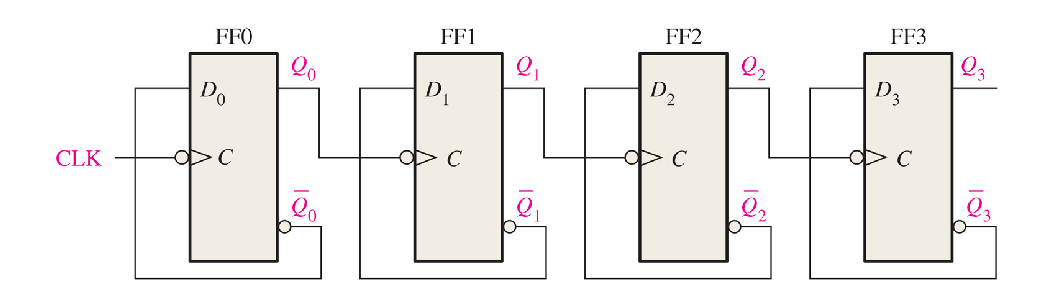
\includegraphics[width=0.49\textwidth]{figures/counter_11.pdf} \\ \vspace{1cm}
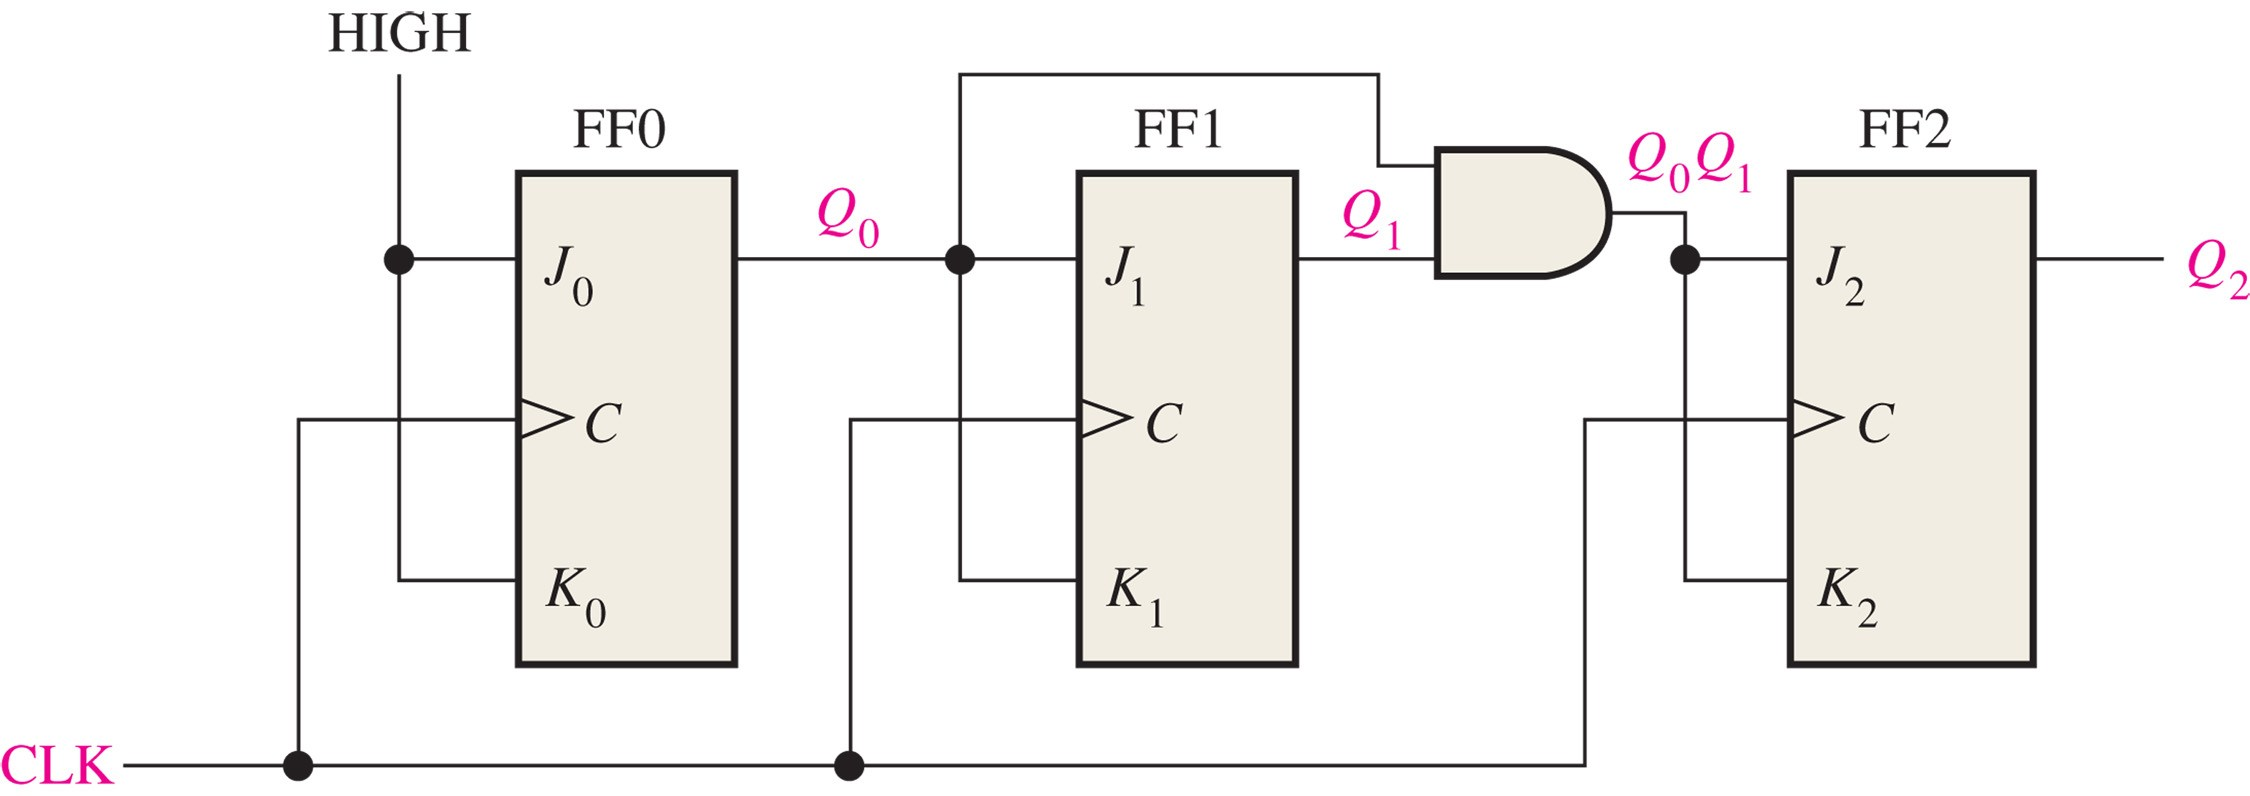
\includegraphics[width=0.49\textwidth]{figures/counter_10.jpg}
\caption{\label{fig:1} (Top) A 4-bit, asynchronous counter, assembled from D flip-flops. (Bottom) A 3-bit, synchronous counter, assembled from JK flip-flops.}
\end{figure}

\end{document}
